% Options for packages loaded elsewhere
\PassOptionsToPackage{unicode}{hyperref}
\PassOptionsToPackage{hyphens}{url}
%
\documentclass[
]{article}
\usepackage{lmodern}
\usepackage{amssymb,amsmath}
\usepackage{ifxetex,ifluatex}
\ifnum 0\ifxetex 1\fi\ifluatex 1\fi=0 % if pdftex
  \usepackage[T1]{fontenc}
  \usepackage[utf8]{inputenc}
  \usepackage{textcomp} % provide euro and other symbols
\else % if luatex or xetex
  \usepackage{unicode-math}
  \defaultfontfeatures{Scale=MatchLowercase}
  \defaultfontfeatures[\rmfamily]{Ligatures=TeX,Scale=1}
\fi
% Use upquote if available, for straight quotes in verbatim environments
\IfFileExists{upquote.sty}{\usepackage{upquote}}{}
\IfFileExists{microtype.sty}{% use microtype if available
  \usepackage[]{microtype}
  \UseMicrotypeSet[protrusion]{basicmath} % disable protrusion for tt fonts
}{}
\makeatletter
\@ifundefined{KOMAClassName}{% if non-KOMA class
  \IfFileExists{parskip.sty}{%
    \usepackage{parskip}
  }{% else
    \setlength{\parindent}{0pt}
    \setlength{\parskip}{6pt plus 2pt minus 1pt}}
}{% if KOMA class
  \KOMAoptions{parskip=half}}
\makeatother
\usepackage{xcolor}
\IfFileExists{xurl.sty}{\usepackage{xurl}}{} % add URL line breaks if available
\IfFileExists{bookmark.sty}{\usepackage{bookmark}}{\usepackage{hyperref}}
\hypersetup{
  pdftitle={Characterising communities and their ecotones with the EcotoneFinder package},
  pdfauthor={Antoine Bagnaro},
  hidelinks,
  pdfcreator={LaTeX via pandoc}}
\urlstyle{same} % disable monospaced font for URLs
\usepackage[margin=1in]{geometry}
\usepackage{color}
\usepackage{fancyvrb}
\newcommand{\VerbBar}{|}
\newcommand{\VERB}{\Verb[commandchars=\\\{\}]}
\DefineVerbatimEnvironment{Highlighting}{Verbatim}{commandchars=\\\{\}}
% Add ',fontsize=\small' for more characters per line
\usepackage{framed}
\definecolor{shadecolor}{RGB}{248,248,248}
\newenvironment{Shaded}{\begin{snugshade}}{\end{snugshade}}
\newcommand{\AlertTok}[1]{\textcolor[rgb]{0.94,0.16,0.16}{#1}}
\newcommand{\AnnotationTok}[1]{\textcolor[rgb]{0.56,0.35,0.01}{\textbf{\textit{#1}}}}
\newcommand{\AttributeTok}[1]{\textcolor[rgb]{0.77,0.63,0.00}{#1}}
\newcommand{\BaseNTok}[1]{\textcolor[rgb]{0.00,0.00,0.81}{#1}}
\newcommand{\BuiltInTok}[1]{#1}
\newcommand{\CharTok}[1]{\textcolor[rgb]{0.31,0.60,0.02}{#1}}
\newcommand{\CommentTok}[1]{\textcolor[rgb]{0.56,0.35,0.01}{\textit{#1}}}
\newcommand{\CommentVarTok}[1]{\textcolor[rgb]{0.56,0.35,0.01}{\textbf{\textit{#1}}}}
\newcommand{\ConstantTok}[1]{\textcolor[rgb]{0.00,0.00,0.00}{#1}}
\newcommand{\ControlFlowTok}[1]{\textcolor[rgb]{0.13,0.29,0.53}{\textbf{#1}}}
\newcommand{\DataTypeTok}[1]{\textcolor[rgb]{0.13,0.29,0.53}{#1}}
\newcommand{\DecValTok}[1]{\textcolor[rgb]{0.00,0.00,0.81}{#1}}
\newcommand{\DocumentationTok}[1]{\textcolor[rgb]{0.56,0.35,0.01}{\textbf{\textit{#1}}}}
\newcommand{\ErrorTok}[1]{\textcolor[rgb]{0.64,0.00,0.00}{\textbf{#1}}}
\newcommand{\ExtensionTok}[1]{#1}
\newcommand{\FloatTok}[1]{\textcolor[rgb]{0.00,0.00,0.81}{#1}}
\newcommand{\FunctionTok}[1]{\textcolor[rgb]{0.00,0.00,0.00}{#1}}
\newcommand{\ImportTok}[1]{#1}
\newcommand{\InformationTok}[1]{\textcolor[rgb]{0.56,0.35,0.01}{\textbf{\textit{#1}}}}
\newcommand{\KeywordTok}[1]{\textcolor[rgb]{0.13,0.29,0.53}{\textbf{#1}}}
\newcommand{\NormalTok}[1]{#1}
\newcommand{\OperatorTok}[1]{\textcolor[rgb]{0.81,0.36,0.00}{\textbf{#1}}}
\newcommand{\OtherTok}[1]{\textcolor[rgb]{0.56,0.35,0.01}{#1}}
\newcommand{\PreprocessorTok}[1]{\textcolor[rgb]{0.56,0.35,0.01}{\textit{#1}}}
\newcommand{\RegionMarkerTok}[1]{#1}
\newcommand{\SpecialCharTok}[1]{\textcolor[rgb]{0.00,0.00,0.00}{#1}}
\newcommand{\SpecialStringTok}[1]{\textcolor[rgb]{0.31,0.60,0.02}{#1}}
\newcommand{\StringTok}[1]{\textcolor[rgb]{0.31,0.60,0.02}{#1}}
\newcommand{\VariableTok}[1]{\textcolor[rgb]{0.00,0.00,0.00}{#1}}
\newcommand{\VerbatimStringTok}[1]{\textcolor[rgb]{0.31,0.60,0.02}{#1}}
\newcommand{\WarningTok}[1]{\textcolor[rgb]{0.56,0.35,0.01}{\textbf{\textit{#1}}}}
\usepackage{graphicx}
\makeatletter
\def\maxwidth{\ifdim\Gin@nat@width>\linewidth\linewidth\else\Gin@nat@width\fi}
\def\maxheight{\ifdim\Gin@nat@height>\textheight\textheight\else\Gin@nat@height\fi}
\makeatother
% Scale images if necessary, so that they will not overflow the page
% margins by default, and it is still possible to overwrite the defaults
% using explicit options in \includegraphics[width, height, ...]{}
\setkeys{Gin}{width=\maxwidth,height=\maxheight,keepaspectratio}
% Set default figure placement to htbp
\makeatletter
\def\fps@figure{htbp}
\makeatother
\setlength{\emergencystretch}{3em} % prevent overfull lines
\providecommand{\tightlist}{%
  \setlength{\itemsep}{0pt}\setlength{\parskip}{0pt}}
\setcounter{secnumdepth}{-\maxdimen} % remove section numbering
\usepackage[font={footnotesize}]{caption}
\ifluatex
  \usepackage{selnolig}  % disable illegal ligatures
\fi
\usepackage[]{biblatex}
\addbibresource{Papers2.bib}

\title{Characterising communities and their ecotones with the
EcotoneFinder package}
\author{Antoine Bagnaro}
\date{2021-02-22}

\begin{document}
\maketitle

{
\setcounter{tocdepth}{2}
\tableofcontents
}
\hypertarget{introduction}{%
\subsection{Introduction}\label{introduction}}

The aim of this vignette is mainly to serve as a tutorial to show how to
use the \emph{EcotoneFinder} package, which implements methods for the
localisation and characterisations of both ecotones and ecological
communities along gradients, in ecosystem-wide representations. The set
of functions present in this package provide a workflow from an initial
data set (typically containing field data) to the extraction of relevant
ecotone and community information and publishable graphical outputs. The
basic organisation of the \emph{EcotoneFinder} package is given in
Figure 1. The rest of this tutorial will be structured
function-by-function, as highlighted by the roman numbers in parenthesis
in Figure 1.

\begin{figure}

{\centering 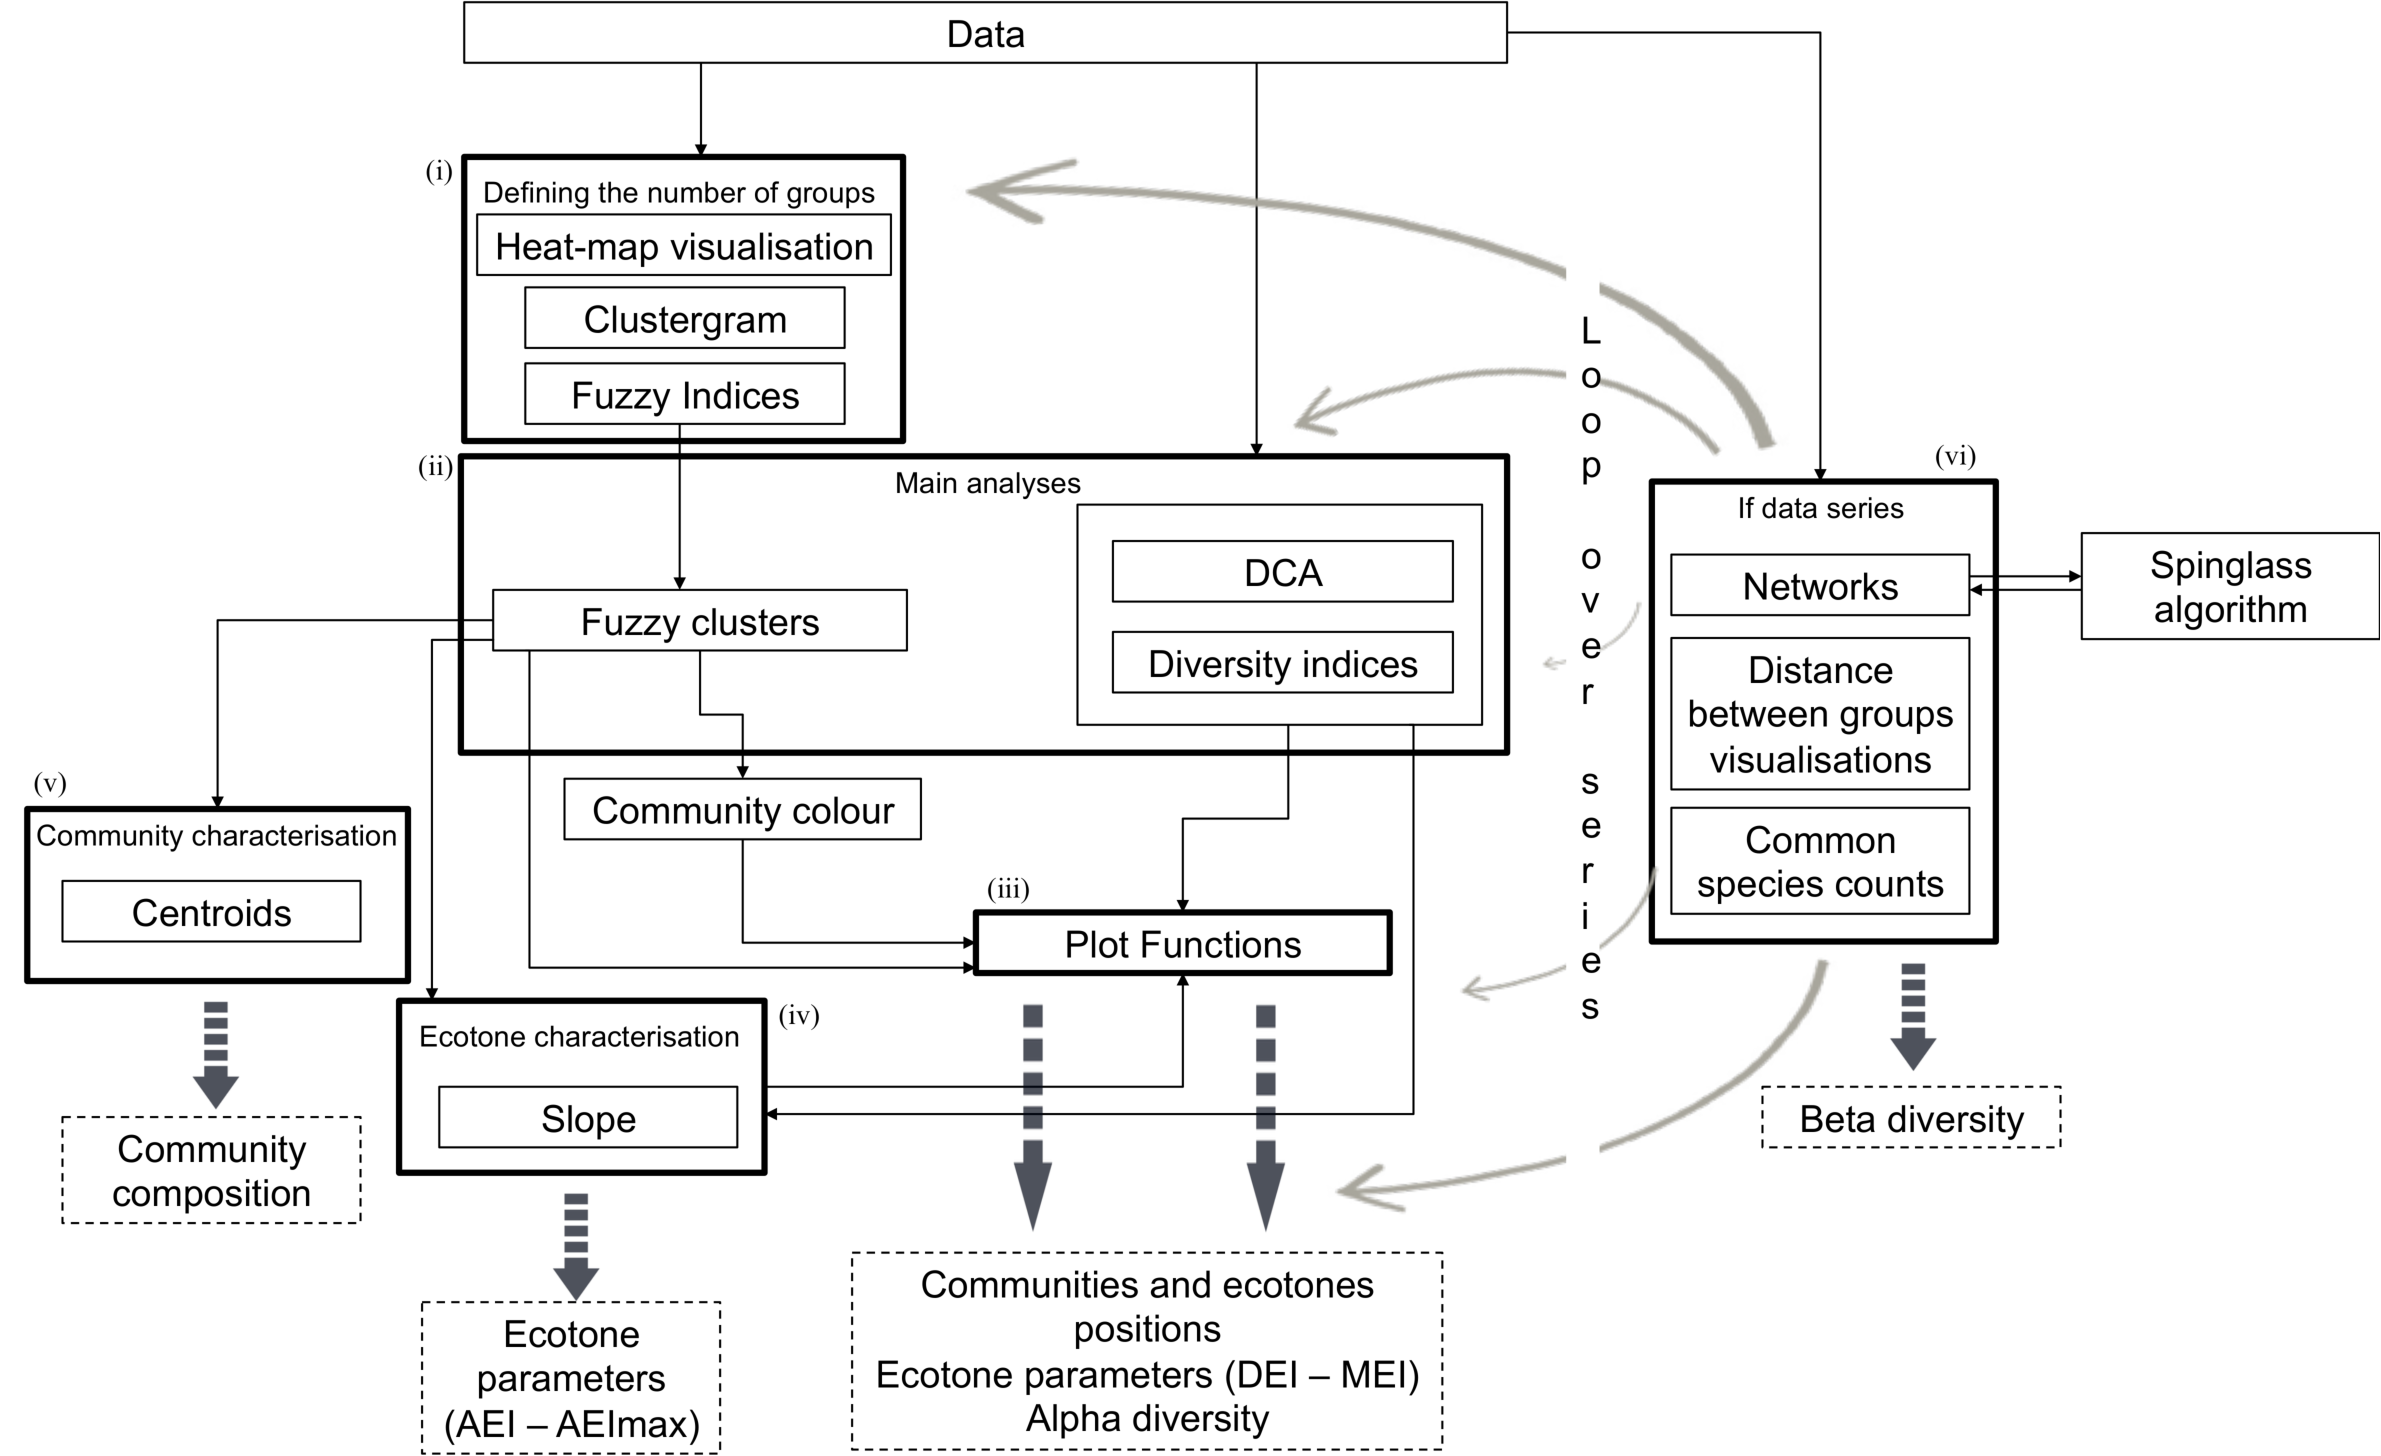
\includegraphics[width=0.85\linewidth]{AnalysesDiagram} 

}

\caption{General organisation chart of the R-package, from raw data to typical outputs. It may be subdivided in several main sections: (i) functions to explore the internal structure of the raw data, (ii) main data analyses for ecotones and communities characterisation, (iii) plotting functions, (iv) functions to extract ecotone parameters, (v) functions to access community compositions and (vi) extensions of these functions for data series.}\label{fig:unnamed-chunk-2}
\end{figure}

First, we start by loading the package:

\begin{Shaded}
\begin{Highlighting}[]
\KeywordTok{library}\NormalTok{(EcotoneFinder)}
\end{Highlighting}
\end{Shaded}

\hypertarget{artificial-data-generation}{%
\subsection{Artificial data
generation:}\label{artificial-data-generation}}

The use of artificial data -- with known patterns -- is a powerful
evaluation method for statistical approaches \autocite{Austin:2007jwa},
as it is not hindered by the unknown nature of the actual relationship
between variables, and by the high level of variability of field data
\autocite{Austin:2007jwa,Schweiger:2016gt}. As a commodity, the
EcotoneFinder package implements two functions to generate artificial
datasets (\texttt{SyntheticData} and \texttt{SyntheticDataSeries}). The
use of artificial data will also provide a practical workflow for the
presentation of the R-package.

The artificial data generates gaussian-shaped species abundance curves,
as equivalent to species response curves \autocite{Whittaker:1967wn},
along the x-axis (which corresponds to the ``distance'' gradient, or
transect). Groups of species form communities by having similar response
curves along the x-axis (Figure 2).

\begin{Shaded}
\begin{Highlighting}[]
\CommentTok{\# 2 Communities {-} 26 species:}
\NormalTok{Community2 \textless{}{-}}\StringTok{ }\KeywordTok{SyntheticData}\NormalTok{(}\DataTypeTok{SpeciesNum =} \DecValTok{26}\NormalTok{, }\DataTypeTok{CommunityNum =} \DecValTok{2}\NormalTok{, }\DataTypeTok{SpCo =} \OtherTok{NULL}\NormalTok{, }
    \DataTypeTok{Length =} \DecValTok{500}\NormalTok{, }\DataTypeTok{Parameters =} \KeywordTok{list}\NormalTok{(}\DataTypeTok{a =} \KeywordTok{c}\NormalTok{(}\DecValTok{60}\NormalTok{, }\DecValTok{60}\NormalTok{), }\DataTypeTok{b =} \KeywordTok{c}\NormalTok{(}\DecValTok{0}\NormalTok{, }\DecValTok{500}\NormalTok{), }\DataTypeTok{c =} \KeywordTok{c}\NormalTok{(}\FloatTok{0.009}\NormalTok{, }
        \FloatTok{0.009}\NormalTok{)), }\DataTypeTok{dev.c =} \FloatTok{0.0024}\NormalTok{, }\DataTypeTok{dev.a =} \DecValTok{25}\NormalTok{, }\DataTypeTok{dev.b =} \DecValTok{30}\NormalTok{, }\DataTypeTok{pal =} \KeywordTok{c}\NormalTok{(}\StringTok{"\#008585"}\NormalTok{, }
        \StringTok{"\#C7522B"}\NormalTok{), }\DataTypeTok{title =} \StringTok{"2 communities"}\NormalTok{)}

\CommentTok{\# 3 Communities {-} 39 species:}
\NormalTok{Community3 \textless{}{-}}\StringTok{ }\KeywordTok{SyntheticData}\NormalTok{(}\DataTypeTok{SpeciesNum =} \DecValTok{39}\NormalTok{, }\DataTypeTok{CommunityNum =} \DecValTok{3}\NormalTok{, }\DataTypeTok{SpCo =} \OtherTok{NULL}\NormalTok{, }
    \DataTypeTok{Length =} \DecValTok{500}\NormalTok{, }\DataTypeTok{Parameters =} \KeywordTok{list}\NormalTok{(}\DataTypeTok{a =} \KeywordTok{c}\NormalTok{(}\DecValTok{60}\NormalTok{, }\DecValTok{60}\NormalTok{, }\DecValTok{60}\NormalTok{), }\DataTypeTok{b =} \KeywordTok{c}\NormalTok{(}\DecValTok{0}\NormalTok{, }\DecValTok{250}\NormalTok{, }\DecValTok{500}\NormalTok{), }
        \DataTypeTok{c =} \KeywordTok{c}\NormalTok{(}\FloatTok{0.015}\NormalTok{, }\FloatTok{0.015}\NormalTok{, }\FloatTok{0.015}\NormalTok{)), }\DataTypeTok{dev.c =} \FloatTok{0.0024}\NormalTok{, }\DataTypeTok{dev.a =} \DecValTok{35}\NormalTok{, }\DataTypeTok{dev.b =} \DecValTok{25}\NormalTok{, }
    \DataTypeTok{pal =} \KeywordTok{c}\NormalTok{(}\StringTok{"\#008585"}\NormalTok{, }\StringTok{"\#B8CDAE"}\NormalTok{, }\StringTok{"\#C7522B"}\NormalTok{), }\DataTypeTok{title =} \StringTok{"3 communities"}\NormalTok{)}
\end{Highlighting}
\end{Shaded}

\begin{figure}
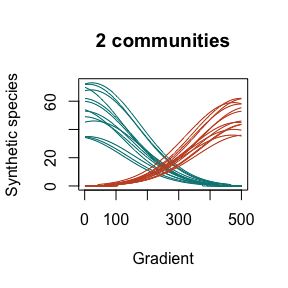
\includegraphics[width=0.5\linewidth]{EcotoneFinder-vignette_files/figure-latex/unnamed-chunk-3-1} 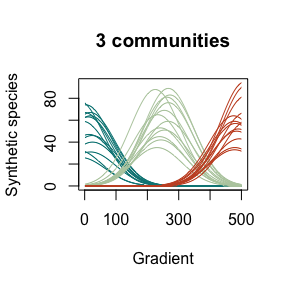
\includegraphics[width=0.5\linewidth]{EcotoneFinder-vignette_files/figure-latex/unnamed-chunk-3-2} \caption{Examples of artificial data with 2 and 3 communities}\label{fig:unnamed-chunk-3}
\end{figure}

\texttt{SpeciesNum} controls the number of curves and
\texttt{CommunityNum} the number of communities. Note that the community
matrices are stored in the \texttt{Community2} and \texttt{Community3}
objects (dataset format). Species curves belonging to the same
communities share the same sets of parameters for their gaussian
response curves (the \texttt{Parameters} argument). The internal
gaussian formula is of the form: \[ae^{-\frac{(x-b)^2}{2c^2}}\] This
simple formula allows for an easy manipulation of the shapes of the
curves. The three parameters, \texttt{a}, \texttt{b} and \texttt{c},
respectively control the height of the curve, the position of its centre
and the steepness of the slopes on both sides (as shown in Figure 3).

\begin{Shaded}
\begin{Highlighting}[]
\CommentTok{\# 2 Communities {-} a = 80 and a = 40:}
\NormalTok{Community2 \textless{}{-}}\StringTok{ }\KeywordTok{SyntheticData}\NormalTok{(}\DataTypeTok{SpeciesNum =} \DecValTok{26}\NormalTok{, }\DataTypeTok{CommunityNum =} \DecValTok{2}\NormalTok{, }\DataTypeTok{SpCo =} \OtherTok{NULL}\NormalTok{, }
    \DataTypeTok{Length =} \DecValTok{500}\NormalTok{, }\DataTypeTok{Parameters =} \KeywordTok{list}\NormalTok{(}\DataTypeTok{a =} \KeywordTok{c}\NormalTok{(}\DecValTok{80}\NormalTok{, }\DecValTok{40}\NormalTok{), }\DataTypeTok{b =} \KeywordTok{c}\NormalTok{(}\DecValTok{0}\NormalTok{, }\DecValTok{500}\NormalTok{), }\DataTypeTok{c =} \KeywordTok{c}\NormalTok{(}\FloatTok{0.009}\NormalTok{, }
        \FloatTok{0.009}\NormalTok{)), }\DataTypeTok{dev.c =} \FloatTok{0.0024}\NormalTok{, }\DataTypeTok{dev.a =} \DecValTok{25}\NormalTok{, }\DataTypeTok{dev.b =} \DecValTok{30}\NormalTok{, }\DataTypeTok{pal =} \KeywordTok{c}\NormalTok{(}\StringTok{"\#008585"}\NormalTok{, }
        \StringTok{"\#C7522B"}\NormalTok{), }\DataTypeTok{title =} \StringTok{"a = 80 and a = 40"}\NormalTok{)}

\CommentTok{\# 2 Communities {-} b = 150 and b = 350:}
\NormalTok{Community2 \textless{}{-}}\StringTok{ }\KeywordTok{SyntheticData}\NormalTok{(}\DataTypeTok{SpeciesNum =} \DecValTok{26}\NormalTok{, }\DataTypeTok{CommunityNum =} \DecValTok{2}\NormalTok{, }\DataTypeTok{SpCo =} \OtherTok{NULL}\NormalTok{, }
    \DataTypeTok{Length =} \DecValTok{500}\NormalTok{, }\DataTypeTok{Parameters =} \KeywordTok{list}\NormalTok{(}\DataTypeTok{a =} \KeywordTok{c}\NormalTok{(}\DecValTok{60}\NormalTok{, }\DecValTok{60}\NormalTok{), }\DataTypeTok{b =} \KeywordTok{c}\NormalTok{(}\DecValTok{100}\NormalTok{, }\DecValTok{400}\NormalTok{), }\DataTypeTok{c =} \KeywordTok{c}\NormalTok{(}\FloatTok{0.009}\NormalTok{, }
        \FloatTok{0.009}\NormalTok{)), }\DataTypeTok{dev.c =} \FloatTok{0.0024}\NormalTok{, }\DataTypeTok{dev.a =} \DecValTok{25}\NormalTok{, }\DataTypeTok{dev.b =} \DecValTok{30}\NormalTok{, }\DataTypeTok{pal =} \KeywordTok{c}\NormalTok{(}\StringTok{"\#008585"}\NormalTok{, }
        \StringTok{"\#C7522B"}\NormalTok{), }\DataTypeTok{title =} \StringTok{"b = 150 and b = 350"}\NormalTok{)}

\CommentTok{\# 2 Communities {-} c = 0.005 and c = 0.012:}
\NormalTok{Community2 \textless{}{-}}\StringTok{ }\KeywordTok{SyntheticData}\NormalTok{(}\DataTypeTok{SpeciesNum =} \DecValTok{26}\NormalTok{, }\DataTypeTok{CommunityNum =} \DecValTok{2}\NormalTok{, }\DataTypeTok{SpCo =} \OtherTok{NULL}\NormalTok{, }
    \DataTypeTok{Length =} \DecValTok{500}\NormalTok{, }\DataTypeTok{Parameters =} \KeywordTok{list}\NormalTok{(}\DataTypeTok{a =} \KeywordTok{c}\NormalTok{(}\DecValTok{60}\NormalTok{, }\DecValTok{60}\NormalTok{), }\DataTypeTok{b =} \KeywordTok{c}\NormalTok{(}\DecValTok{0}\NormalTok{, }\DecValTok{500}\NormalTok{), }\DataTypeTok{c =} \KeywordTok{c}\NormalTok{(}\FloatTok{0.005}\NormalTok{, }
        \FloatTok{0.012}\NormalTok{)), }\DataTypeTok{dev.c =} \FloatTok{0.0024}\NormalTok{, }\DataTypeTok{dev.a =} \DecValTok{25}\NormalTok{, }\DataTypeTok{dev.b =} \DecValTok{30}\NormalTok{, }\DataTypeTok{pal =} \KeywordTok{c}\NormalTok{(}\StringTok{"\#008585"}\NormalTok{, }
        \StringTok{"\#C7522B"}\NormalTok{), }\DataTypeTok{title =} \StringTok{"c = 0.005 and c = 0.012"}\NormalTok{)}
\end{Highlighting}
\end{Shaded}

\begin{figure}
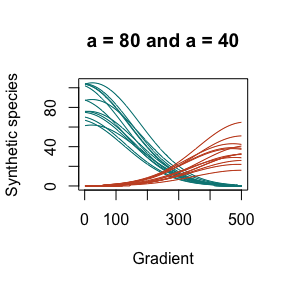
\includegraphics[width=0.33\linewidth]{EcotoneFinder-vignette_files/figure-latex/unnamed-chunk-4-1} 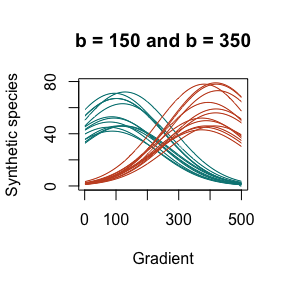
\includegraphics[width=0.33\linewidth]{EcotoneFinder-vignette_files/figure-latex/unnamed-chunk-4-2} 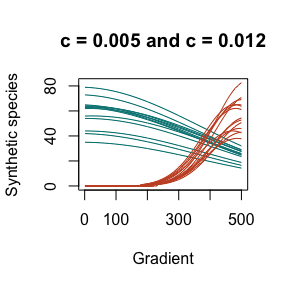
\includegraphics[width=0.33\linewidth]{EcotoneFinder-vignette_files/figure-latex/unnamed-chunk-4-3} \caption{Examples of artificial data with different gaussian parameters}\label{fig:unnamed-chunk-4}
\end{figure}

So far, the \texttt{SpCo} argument has been left \texttt{NULL}. By
default, the \texttt{SyntheticData} function equally partition the
species in the different communities (in our example it means that --
out of 26 species -- 13 are put in the first community, and 13 in the
second). The \texttt{SpCo} argument (meaning Species/Community) allows
for user-defined species partioning. Another set of arguments,
\texttt{dev.a}, \texttt{dev.b}, and \texttt{dev.c}, allow for a certain
amount of deviation around the given parameters values, to produce more
or less identical species curves for each community. The gaussian
parameters for each curves are then chosen randomly (via the
\texttt{sample()} function) in the interval
\([Parameter - dev.value ; Parameter + dev.value]\) \textbackslash{}
Playing with these different arguments allows for the generation of
diverse sets of artificial data (Figure 4).

\begin{Shaded}
\begin{Highlighting}[]
\CommentTok{\# 2 Communities with unequal species numbers:}
\NormalTok{Community2 \textless{}{-}}\StringTok{ }\KeywordTok{SyntheticData}\NormalTok{(}\DataTypeTok{SpeciesNum =} \DecValTok{30}\NormalTok{, }\DataTypeTok{CommunityNum =} \DecValTok{2}\NormalTok{, }\DataTypeTok{SpCo =} \KeywordTok{c}\NormalTok{(}\DecValTok{10}\NormalTok{, }
    \DecValTok{20}\NormalTok{), }\DataTypeTok{Length =} \DecValTok{500}\NormalTok{, }\DataTypeTok{Parameters =} \KeywordTok{list}\NormalTok{(}\DataTypeTok{a =} \KeywordTok{c}\NormalTok{(}\DecValTok{60}\NormalTok{, }\DecValTok{60}\NormalTok{), }\DataTypeTok{b =} \KeywordTok{c}\NormalTok{(}\DecValTok{0}\NormalTok{, }\DecValTok{500}\NormalTok{), }
    \DataTypeTok{c =} \KeywordTok{c}\NormalTok{(}\FloatTok{0.009}\NormalTok{, }\FloatTok{0.009}\NormalTok{)), }\DataTypeTok{dev.c =} \FloatTok{0.0024}\NormalTok{, }\DataTypeTok{dev.a =} \DecValTok{25}\NormalTok{, }\DataTypeTok{dev.b =} \DecValTok{30}\NormalTok{, }\DataTypeTok{pal =} \KeywordTok{c}\NormalTok{(}\StringTok{"\#008585"}\NormalTok{, }
    \StringTok{"\#C7522B"}\NormalTok{), }\DataTypeTok{title =} \StringTok{"Unequal species numbers"}\NormalTok{)}

\CommentTok{\# Adding parameter deviations:}
\NormalTok{Community2 \textless{}{-}}\StringTok{ }\KeywordTok{SyntheticData}\NormalTok{(}\DataTypeTok{SpeciesNum =} \DecValTok{30}\NormalTok{, }\DataTypeTok{CommunityNum =} \DecValTok{2}\NormalTok{, }\DataTypeTok{SpCo =} \OtherTok{NULL}\NormalTok{, }
    \DataTypeTok{Length =} \DecValTok{500}\NormalTok{, }\DataTypeTok{Parameters =} \KeywordTok{list}\NormalTok{(}\DataTypeTok{a =} \KeywordTok{c}\NormalTok{(}\DecValTok{60}\NormalTok{, }\DecValTok{60}\NormalTok{), }\DataTypeTok{b =} \KeywordTok{c}\NormalTok{(}\DecValTok{0}\NormalTok{, }\DecValTok{500}\NormalTok{), }\DataTypeTok{c =} \KeywordTok{c}\NormalTok{(}\FloatTok{0.009}\NormalTok{, }
        \FloatTok{0.009}\NormalTok{)), }\DataTypeTok{dev.c =} \FloatTok{0.005}\NormalTok{, }\DataTypeTok{dev.a =} \DecValTok{50}\NormalTok{, }\DataTypeTok{dev.b =} \DecValTok{60}\NormalTok{, }\DataTypeTok{pal =} \KeywordTok{c}\NormalTok{(}\StringTok{"\#008585"}\NormalTok{, }
        \StringTok{"\#C7522B"}\NormalTok{), }\DataTypeTok{title =} \StringTok{"Parameter deviation"}\NormalTok{)}

\CommentTok{\# Adding complexity:}
\NormalTok{Community2 \textless{}{-}}\StringTok{ }\KeywordTok{SyntheticData}\NormalTok{(}\DataTypeTok{SpeciesNum =} \DecValTok{60}\NormalTok{, }\DataTypeTok{CommunityNum =} \DecValTok{4}\NormalTok{, }\DataTypeTok{SpCo =} \KeywordTok{c}\NormalTok{(}\DecValTok{20}\NormalTok{, }
    \DecValTok{10}\NormalTok{, }\DecValTok{10}\NormalTok{, }\DecValTok{20}\NormalTok{), }\DataTypeTok{Length =} \DecValTok{500}\NormalTok{, }\DataTypeTok{Parameters =} \KeywordTok{list}\NormalTok{(}\DataTypeTok{a =} \KeywordTok{c}\NormalTok{(}\DecValTok{60}\NormalTok{, }\DecValTok{30}\NormalTok{, }\DecValTok{40}\NormalTok{, }\DecValTok{70}\NormalTok{), }
    \DataTypeTok{b =} \KeywordTok{c}\NormalTok{(}\DecValTok{0}\NormalTok{, }\DecValTok{0}\NormalTok{, }\DecValTok{500}\NormalTok{, }\DecValTok{500}\NormalTok{), }\DataTypeTok{c =} \KeywordTok{c}\NormalTok{(}\FloatTok{0.015}\NormalTok{, }\FloatTok{0.008}\NormalTok{, }\FloatTok{0.007}\NormalTok{, }\FloatTok{0.01}\NormalTok{)), }\DataTypeTok{dev.c =} \FloatTok{0.0024}\NormalTok{, }
    \DataTypeTok{dev.a =} \DecValTok{25}\NormalTok{, }\DataTypeTok{dev.b =} \DecValTok{30}\NormalTok{, }\DataTypeTok{pal =} \KeywordTok{c}\NormalTok{(}\StringTok{"\#008585"}\NormalTok{, }\StringTok{"\#AAC1A8"}\NormalTok{, }\StringTok{"\#D58545"}\NormalTok{, }\StringTok{"\#C7522B"}\NormalTok{), }
    \DataTypeTok{title =} \StringTok{"Pools of species inside community types"}\NormalTok{)}
\end{Highlighting}
\end{Shaded}

\begin{figure}
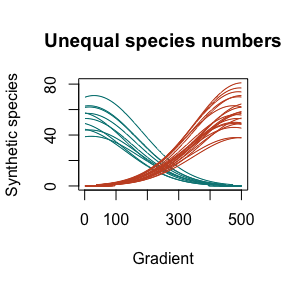
\includegraphics[width=0.33\linewidth]{EcotoneFinder-vignette_files/figure-latex/unnamed-chunk-5-1} 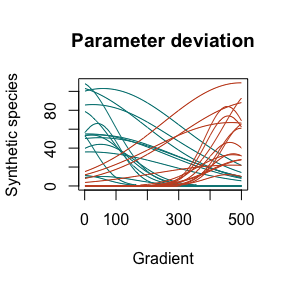
\includegraphics[width=0.33\linewidth]{EcotoneFinder-vignette_files/figure-latex/unnamed-chunk-5-2} 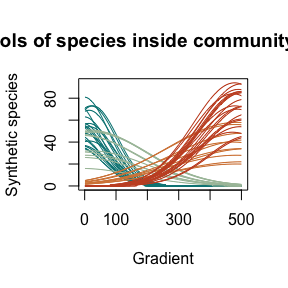
\includegraphics[width=0.33\linewidth]{EcotoneFinder-vignette_files/figure-latex/unnamed-chunk-5-3} \caption{Control of the number of species per communities, of the gaussian parameter deviations and of particular groups of species in community types.}\label{fig:unnamed-chunk-5}
\end{figure}

Lastly, the \texttt{SyntheticDataSeries} function simplifies the
generation of series of artificial data with common characteristics. It
is an automated way to loop over the \texttt{SyntheticData} function,
while controling (to a cerain extent) the kind of changes that are
affecting the data over the series. Particularly, the number of species
per artificial community can vary inside a specified interval (for
instance, to account for the loss or gain of seasonal species over a
time series), and the position of the succesive communities can be set
to move along the gradient (to mimic, for instance, the gradual
displacement of an hypothetical environmental gradient). This can
notably be done with the \texttt{displacement}parameter and a matrix
specifying the desired changes (direction and values) along the x-axis
for each community (Figure 5).

\begin{Shaded}
\begin{Highlighting}[]
\CommentTok{\#\# Displacement matrix:}
\NormalTok{disp \textless{}{-}}\StringTok{ }\KeywordTok{matrix}\NormalTok{(}\DataTypeTok{data =} \KeywordTok{c}\NormalTok{(}\DecValTok{0}\NormalTok{, }\DecValTok{0}\NormalTok{, }\DecValTok{0}\NormalTok{, }\DecValTok{0}\NormalTok{, }\DecValTok{35}\NormalTok{, }\FloatTok{{-}7e{-}04}\NormalTok{, }\DecValTok{0}\NormalTok{, }\DecValTok{10}\NormalTok{, }\DecValTok{0}\NormalTok{), }\DataTypeTok{nrow =} \DecValTok{3}\NormalTok{, }\DataTypeTok{ncol =} \DecValTok{3}\NormalTok{)}

\CommentTok{\#\#\# Series:}
\NormalTok{Series \textless{}{-}}\StringTok{ }\KeywordTok{SyntheticDataSeries}\NormalTok{(}\DataTypeTok{CommunityPool =} \DecValTok{60}\NormalTok{, }\DataTypeTok{CommunityNum =} \DecValTok{3}\NormalTok{, }\DataTypeTok{Length =} \DecValTok{500}\NormalTok{, }
    \DataTypeTok{SeriesNum =} \DecValTok{6}\NormalTok{, }\DataTypeTok{replacement =} \OtherTok{FALSE}\NormalTok{, }\DataTypeTok{SpCo =} \KeywordTok{c}\NormalTok{(}\DecValTok{15}\NormalTok{, }\DecValTok{15}\NormalTok{, }\DecValTok{30}\NormalTok{), }\DataTypeTok{Parameters =} \KeywordTok{list}\NormalTok{(}\DataTypeTok{a =} \KeywordTok{c}\NormalTok{(}\DecValTok{60}\NormalTok{, }
        \DecValTok{60}\NormalTok{, }\DecValTok{60}\NormalTok{), }\DataTypeTok{b =} \KeywordTok{c}\NormalTok{(}\OperatorTok{{-}}\DecValTok{50}\NormalTok{, }\DecValTok{{-}50}\NormalTok{, }\DecValTok{400}\NormalTok{), }\DataTypeTok{c =} \KeywordTok{c}\NormalTok{(}\FloatTok{0.01}\NormalTok{, }\FloatTok{0.01}\NormalTok{, }\FloatTok{0.01}\NormalTok{)), }\DataTypeTok{dev.a =} \DecValTok{30}\NormalTok{, }
    \DataTypeTok{dev.b =} \DecValTok{40}\NormalTok{, }\DataTypeTok{dev.c =} \DecValTok{0}\NormalTok{, }\DataTypeTok{displacement =}\NormalTok{ disp, }\DataTypeTok{pal =} \KeywordTok{c}\NormalTok{(}\KeywordTok{rep}\NormalTok{(}\StringTok{"\#008585"}\NormalTok{, }
        \DecValTok{15}\NormalTok{), }\KeywordTok{rep}\NormalTok{(}\StringTok{"\#E6C186"}\NormalTok{, }\DecValTok{15}\NormalTok{), }\KeywordTok{rep}\NormalTok{(}\StringTok{"\#C7522B"}\NormalTok{, }\DecValTok{30}\NormalTok{)))}
\end{Highlighting}
\end{Shaded}

\begin{figure}
\includegraphics[width=0.33\linewidth]{EcotoneFinder-vignette_files/figure-latex/unnamed-chunk-6-1} \includegraphics[width=0.33\linewidth]{EcotoneFinder-vignette_files/figure-latex/unnamed-chunk-6-2} \includegraphics[width=0.33\linewidth]{EcotoneFinder-vignette_files/figure-latex/unnamed-chunk-6-3} \includegraphics[width=0.33\linewidth]{EcotoneFinder-vignette_files/figure-latex/unnamed-chunk-6-4} \includegraphics[width=0.33\linewidth]{EcotoneFinder-vignette_files/figure-latex/unnamed-chunk-6-5} \includegraphics[width=0.33\linewidth]{EcotoneFinder-vignette_files/figure-latex/unnamed-chunk-6-6} \caption{Time series with displacement: part of the first community (left) advances toward the right-end of the gradient by 35 gradient units per series, as if reacting to a moving environmental variable. The last community also withdraw even further to the right, but slower (10 gradient units per series).}\label{fig:unnamed-chunk-6}
\end{figure}

Now that we have generated some artificial community data, we can
proceed to their analyses.

\hypertarget{internal-structure-of-the-data}{%
\subsection{Internal structure of the
data:}\label{internal-structure-of-the-data}}

One of the recurrent (and vexing) problem encounterd by community
ecologists is the determination of the ``correct'' number of groups in
their data -- in our case, the actual number of communities that have
been sampled. This can be assessed \emph{à-priori} when delineations
between community types are visually obvious (e.g.~between forests and
agricultural lands), or when the number of groups are decided based on
standard protocols (e.g.~to fit data into pre-existing categories). Many
stuations, however, are harder to resolve, either due to the size of the
organisms (making visual assessments impossible), the existance of
closely related groups (making the classification of near-boundary
objects unsactifactory), or the existance of important mismatches
between pre-existing classifications and the reality (driving the
necessity to re-evaluate them).\textbackslash{} A number of approaches
have been proposed over the years to address these issues, with
constrasted results when confronted with the typically high internal
variability of ecological field data. Recent years have seen promising
advances, notably in the field of machine learning. These new approaches
will undoubtly become more and more available over the years. The
\texttt{DistEco} function only implements basic methods to explore the
internal structure of data (based on distance matrix computation,
network analyses and clustergram), to help the decision process. We will
review them in this section, but it is advised to reach out for more
recent approaches if problems persist. \textbackslash{} Distance
matrices can be easilly visualised with heat-maps. In such
representations, groups of more closely related datapoints appear along
the diagonal of the heat-map, forming similarly coloured squares (Fig.
6). The main branches of the hierarchical trees on the sides of the
heat-maps also segregate the data in similar ways.They are often easier
to interpret than the heat-maps themselves when the internal variability
of the data is high. In these situations, the computation of networks
from the raw community data may considerably help -- particularly as
robust statistical tools exist to test for the existance of network
communities (i.e.~groups of nodes that are consistently related,
independantly of network typology). In our case, these network
communities may correspond to actual ecological communities (Fig. 6).
\textbackslash{}

\begin{Shaded}
\begin{Highlighting}[]
\CommentTok{\# 2 Communities {-} 26 species:}
\NormalTok{Community2 \textless{}{-}}\StringTok{ }\KeywordTok{SyntheticData}\NormalTok{(}\DataTypeTok{SpeciesNum =} \DecValTok{26}\NormalTok{, }\DataTypeTok{CommunityNum =} \DecValTok{2}\NormalTok{, }\DataTypeTok{SpCo =} \OtherTok{NULL}\NormalTok{, }
    \DataTypeTok{Length =} \DecValTok{500}\NormalTok{, }\DataTypeTok{Parameters =} \KeywordTok{list}\NormalTok{(}\DataTypeTok{a =} \KeywordTok{c}\NormalTok{(}\DecValTok{60}\NormalTok{, }\DecValTok{60}\NormalTok{), }\DataTypeTok{b =} \KeywordTok{c}\NormalTok{(}\DecValTok{0}\NormalTok{, }\DecValTok{500}\NormalTok{), }\DataTypeTok{c =} \KeywordTok{c}\NormalTok{(}\FloatTok{0.009}\NormalTok{, }
        \FloatTok{0.009}\NormalTok{)), }\DataTypeTok{dev.c =} \FloatTok{0.0024}\NormalTok{, }\DataTypeTok{dev.a =} \DecValTok{25}\NormalTok{, }\DataTypeTok{dev.b =} \DecValTok{30}\NormalTok{, }\DataTypeTok{pal =} \KeywordTok{c}\NormalTok{(}\StringTok{"\#008585"}\NormalTok{, }
        \StringTok{"\#C7522B"}\NormalTok{), }\DataTypeTok{title =} \StringTok{"2 communities"}\NormalTok{)}

\CommentTok{\# 3 Communities {-} 39 species:}
\NormalTok{Community3 \textless{}{-}}\StringTok{ }\KeywordTok{SyntheticData}\NormalTok{(}\DataTypeTok{SpeciesNum =} \DecValTok{39}\NormalTok{, }\DataTypeTok{CommunityNum =} \DecValTok{3}\NormalTok{, }\DataTypeTok{SpCo =} \OtherTok{NULL}\NormalTok{, }
    \DataTypeTok{Length =} \DecValTok{500}\NormalTok{, }\DataTypeTok{Parameters =} \KeywordTok{list}\NormalTok{(}\DataTypeTok{a =} \KeywordTok{c}\NormalTok{(}\DecValTok{60}\NormalTok{, }\DecValTok{60}\NormalTok{, }\DecValTok{60}\NormalTok{), }\DataTypeTok{b =} \KeywordTok{c}\NormalTok{(}\DecValTok{0}\NormalTok{, }\DecValTok{250}\NormalTok{, }\DecValTok{500}\NormalTok{), }
        \DataTypeTok{c =} \KeywordTok{c}\NormalTok{(}\FloatTok{0.015}\NormalTok{, }\FloatTok{0.015}\NormalTok{, }\FloatTok{0.015}\NormalTok{)), }\DataTypeTok{dev.c =} \FloatTok{0.0024}\NormalTok{, }\DataTypeTok{dev.a =} \DecValTok{35}\NormalTok{, }\DataTypeTok{dev.b =} \DecValTok{25}\NormalTok{, }
    \DataTypeTok{pal =} \KeywordTok{c}\NormalTok{(}\StringTok{"\#008585"}\NormalTok{, }\StringTok{"\#B8CDAE"}\NormalTok{, }\StringTok{"\#C7522B"}\NormalTok{), }\DataTypeTok{title =} \StringTok{"3 communities"}\NormalTok{)}

\CommentTok{\# Heat maps:}
\NormalTok{HeatMap2 \textless{}{-}}\StringTok{ }\KeywordTok{DistEco}\NormalTok{(Community2[, }\DecValTok{2}\OperatorTok{:}\KeywordTok{ncol}\NormalTok{(Community2)], }\DataTypeTok{transpose =}\NormalTok{ T, }\DataTypeTok{symm =}\NormalTok{ F, }
    \DataTypeTok{plot =} \KeywordTok{c}\NormalTok{(}\StringTok{"heatmap"}\NormalTok{))}
\NormalTok{HeatMap3 \textless{}{-}}\StringTok{ }\KeywordTok{DistEco}\NormalTok{(Community3[, }\DecValTok{2}\OperatorTok{:}\KeywordTok{ncol}\NormalTok{(Community3)], }\DataTypeTok{transpose =}\NormalTok{ T, }\DataTypeTok{symm =}\NormalTok{ F, }
    \DataTypeTok{plot =} \KeywordTok{c}\NormalTok{(}\StringTok{"heatmap"}\NormalTok{))}

\CommentTok{\# Networks (with spinglass algorithm for statistical communities):}
\NormalTok{Network2 \textless{}{-}}\StringTok{ }\KeywordTok{DistEco}\NormalTok{(Community2[, }\DecValTok{2}\OperatorTok{:}\KeywordTok{ncol}\NormalTok{(Community2)], }\DataTypeTok{transpose =}\NormalTok{ T, }\DataTypeTok{symm =}\NormalTok{ F, }
    \DataTypeTok{plot =} \KeywordTok{c}\NormalTok{(}\StringTok{"network"}\NormalTok{), }\DataTypeTok{spinglass =}\NormalTok{ T, }\DataTypeTok{run =} \DecValTok{5}\NormalTok{, }\DataTypeTok{spinglass.groups =} \KeywordTok{c}\NormalTok{(}\StringTok{"rounded"}\NormalTok{))}
\NormalTok{Network3 \textless{}{-}}\StringTok{ }\KeywordTok{DistEco}\NormalTok{(Community3[, }\DecValTok{2}\OperatorTok{:}\KeywordTok{ncol}\NormalTok{(Community3)], }\DataTypeTok{transpose =}\NormalTok{ T, }\DataTypeTok{symm =}\NormalTok{ F, }
    \DataTypeTok{plot =} \KeywordTok{c}\NormalTok{(}\StringTok{"network"}\NormalTok{), }\DataTypeTok{spinglass =}\NormalTok{ T, }\DataTypeTok{run =} \DecValTok{5}\NormalTok{, }\DataTypeTok{spinglass.groups =} \KeywordTok{c}\NormalTok{(}\StringTok{"rounded"}\NormalTok{))}
\end{Highlighting}
\end{Shaded}

\begin{figure}
\includegraphics[width=0.5\linewidth]{EcotoneFinder-vignette_files/figure-latex/unnamed-chunk-7-1} \includegraphics[width=0.5\linewidth]{EcotoneFinder-vignette_files/figure-latex/unnamed-chunk-7-2} \includegraphics[width=0.5\linewidth]{EcotoneFinder-vignette_files/figure-latex/unnamed-chunk-7-3} \includegraphics[width=0.5\linewidth]{EcotoneFinder-vignette_files/figure-latex/unnamed-chunk-7-4} \includegraphics[width=0.5\linewidth]{EcotoneFinder-vignette_files/figure-latex/unnamed-chunk-7-5} \includegraphics[width=0.5\linewidth]{EcotoneFinder-vignette_files/figure-latex/unnamed-chunk-7-6} \caption{Heatmaps and Networks, based on the example artificial communities presented above in Fig. 2}\label{fig:unnamed-chunk-7}
\end{figure}

\hypertarget{community-detection-along-gradients}{%
\subsection{Community detection along
gradients:}\label{community-detection-along-gradients}}

\hypertarget{detrended-correspondance-analyses-dca}{%
\paragraph{Detrended Correspondance Analyses
(DCA):}\label{detrended-correspondance-analyses-dca}}

Detrended Correspondance Analyses (DCA) were developped by
\autocite{Hill:1980wk}, to circumvent some of the shortcomings of
Correspondance Analyses (CA), and in particular, the distortion of the
ecological gradients by the arch effect. This is done through
detrending, a method that centres the second axis of the CA on zero
(described in \autocite{Gauch:1982tu}. More relevant for ecotonal
studies, the distortion of the gradient is corrected by rescaling, which
makes the beta diversity constant (per axis unit). In other words, for
three samples A, B, and C, if the distance (in the ordination space)
between A and C is twice as much as the distance between A and B, then
beta diversity is effectively twice as much between A and C than between
A and B -- regardless of the position of the samples over geographical
space. This property of DCA enables it to consistently capture community
variability along spatial gradients \autocite{Feilhauer:2009uz}.

\printbibliography

\end{document}
